\section{La gerarchia di Von Neumann e l'assioma di buona fondazione}
Insiemi come questi sono (forse?) mostri indesiderabili:

\begin{figure}[H]
	\centering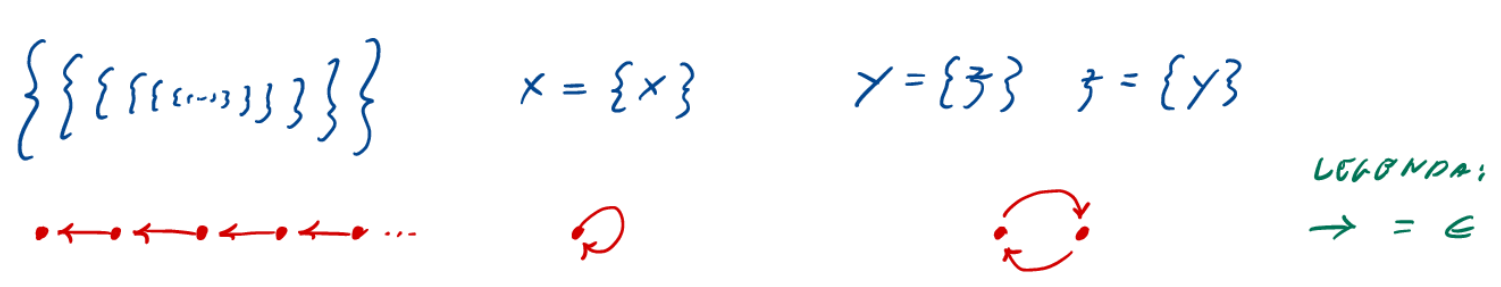
\includegraphics[width = 11.5cm]{immagini/mostri.png}
\end{figure}

Desideriamo dimostrare, intanto, che, a patto che gli assiomi della teoria degli insiemi non si contraddicano - nel qual caso dimostrerebbero qualunque cosa - essi NON dimostrano l'esistenza di insiemi del genere.\\
\textbf{\underline{Startegia}}: costruiamo un universo insiemistico $V_*$, che è una classe propria, al cui interno gli assiomi sono veri, e che, tuttavia, non contiene quella robaccia.

\begin{definition}[Gerarchia di \href{https://en.wikipedia.org/wiki/John_von_Neumann}{\textcolor{purple}{Von Neumann}}]
	Costruiamo per ricorsione transfinita la \vocab{gerarchia di Von Neumann} come segue:
	\begin{align*}
		&V_0 = \emptyset \\
		&V_{s(\alpha)} = \ps(V_\alpha) \\
		&V_\lambda = \bigcup\{V_\alpha | \alpha < \lambda\} \; \text{per $\lambda$ limite}
	\end{align*}
	La classe $V_*$ è l'unione degli insiemi $V_\alpha$, formalmente:
	\[ x \in V_* \Mydef \exists \alpha \in \Ord \; x \in V_\alpha
		\]
	(dove $V_*$ è una classe perché l'abbiamo definita come la formula al RHS).
\end{definition}

\begin{lemma}[$V_\alpha$ è transitivo]
	$\forall \alpha \in \Ord$ $V_\alpha$ è un insieme transitivo.
\end{lemma}

\begin{proof}
	Procediamo per induzione transfinita.
	\begin{itemize}
		\item[$\boxed{\text{caso $V_0$}}$] Immediato perché $\emptyset$ è un insieme transitivo a vuoto.
		\item[$\boxed{\text{caso successore}}$] Supponiamo che $V_\alpha$ sia un insieme transitivo e dimostriamo che
		anche $V_{s(\alpha)}$ lo è. Dato $x \in V_{s(\alpha)}$ vogliamo arrivare a dire che $x \subseteq V_{s(\alpha)}$ (o equivalentemente
		che $\forall y \in x \; y \in V_{s(\alpha)}$). Per farlo ci basta osservare che:
		\[ x \in V_{s(\alpha)} = \ps(V_\alpha) \implies x \subseteq V_\alpha
			\]
		ora, poiché $V_\alpha$ è transitivo per ipotesi induttiva, tutti gli elementi di $x$ sono a loro volta sottoinsiemi di $V_\alpha$ [cioè essendo elementi di un sottoinsieme sono in primis elementi di $V_\alpha$, poi per la transitività
		di quest'ultimo sappiamo che tutti gli elementi sono sottoinsiemi]\footnote{Attenzione al fatto che transitivo non dice che i sottoinsiemi sono necessariamente elementi, quindi $x$ non è detto sia un elemento di $V_\alpha$, ma è un sottoinsieme
		di $V_\alpha$ e questo ci basta.}, ovvero $\forall y \in x \; y \subseteq V_\alpha \implies \forall y \in x \; y \in \ps(V_\alpha) = V_{s(\alpha)}$, pertanto è verificata la definizione di transitività in $V_{s(\alpha)}$.
		\item[$\boxed{\text{caso limite}}$] Assumiamo per ipotesi induttiva che $V_\alpha$ sia transitivo per ogni $\alpha < \lambda$. Per definizione:
		\[ x \in V_\lambda \implies x \in V_\alpha
			\]
		per qualche $\alpha < \lambda$, ma allora per ipotesi induttiva $x \subseteq V_\alpha \subseteq V_\lambda$ [la seconda uguaglianza è la definizione nel caso limite].
	\end{itemize}
\end{proof}

\begin{corollary}[$V_*$ è una classe transitiva]
	$V_*$ è una \vocab{classe transitiva}, ossia $\forall x \in V_* \; x \subseteq V_*$.
\end{corollary}

\begin{proof}
	Se $x \in V_*$, allora per definizione $x \in V_\alpha$ per qualche $\alpha \in \Ord$, quindi per la proposizione sopra $x \subseteq V_\alpha$, ovvero $x$ è un insieme di cose che soddisfano il predicato che definisce $V_*$, quindi $x \subseteq V_*$.
\end{proof}

\begin{lemma}[``Ordinamento'' di $V_*$]
	$\forall \alpha, \beta \in \Ord \; \alpha < \beta \rightarrow V_\alpha \subseteq V_\beta$.
\end{lemma}

\begin{proof}
	Procediamo per induzione transfinita su $\beta$.
	\begin{itemize}
		\item[$\boxed{\text{caso $\beta = 0$}}$] Vero a vuoto.
		\item[$\boxed{\text{caso successore}}$] Dobbiamo dimostrare che $\forall \alpha < s(\beta) \; V_\alpha \subseteq V_{s(\beta)}$, e abbiamo per ipotesi induttiva $\forall \alpha < \beta \; V_\alpha \subseteq V_\beta$.
		Siccome $\alpha < s(\beta) \leftrightarrow \alpha \leq \beta$, si danno due casi, e $\alpha = \beta$ è banalmente vero, dunque abbiamo $\alpha < \beta$, quindi per ipotesi induttiva $V_\alpha \subseteq V_\beta$.\\
		Per la definizione ricorsiva si ha $V_\alpha \subseteq V_\beta \implies V_\alpha \in \ps(V_\beta) = V_{s(\beta)}$, ma, per la transitività di quest'ultimo, si ottiene che $V_\alpha \subseteq V_{s(\beta)}$.
		\item[$\boxed{\text{caso limite}}$] Abbiamo per ipotesi che $\forall \alpha < \beta < \lambda \; V_\alpha \subseteq V_\beta$, e vogliamo dimostrare che $\forall \alpha < \lambda \; V_\alpha \subseteq V_\beta$. Questo segue facilmente dall'ipotesi e dalla definizione,
		infatti, $V_\lambda = \bigcup\{V_\gamma | \gamma < \lambda\}$, ciò significa che $V_\beta \subseteq V_\lambda$ per ogni $\beta < \lambda$, unendo ciò all'ipotesi si ottiene la tesi, $\forall \alpha < \beta < \lambda \; V_\alpha \overset{\text{Hp. indutt.}}{\subseteq} V_\beta \overset{\text{def. $V_\lambda$}}{\subseteq} V_\lambda \implies \forall \alpha < \lambda\; V_\alpha \subseteq V_\lambda$.
		\footnote{In realtà si poteva concludere anche senza usare l'ipotesi induttiva, in quanto $\alpha < \lambda \implies V_\alpha \subseteq \bigcup{V_\gamma | \gamma < \lambda} = V_\lambda \implies V_\alpha \subseteq V_\lambda$.}
	\end{itemize}
\end{proof}

\begin{lemma}[Ogni ordinale è contenuto nella sua immagine in $V_*$]
	$\forall \alpha \in \Ord \; \alpha \subseteq V_\alpha$.
\end{lemma}

\begin{proof}
	Come al solito per induzione transfinita.
	\begin{itemize}
		\item[$\boxed{\text{caso $0$}}$] $0 \subseteq V_0 = \emptyset$, vera [perché scrivendo estesamente la formula insiemistica si ha una premessa falsa].
		\item[$\boxed{\text{caso successore}}$] Supponiamo che $\alpha \subseteq V_\alpha$ e dimostriamo che $s(\alpha) \subseteq V_{s(\alpha)}$. Osserviamo che dall'ipotesi si ha:
		\[ \alpha \subseteq V_\alpha \implies \alpha \in \ps(V_\alpha) = V_{s(\alpha)} \overset{\text{transitività}}{\implies} \alpha \subseteq V_{s(\alpha)}
			\]
		inoltre $\alpha \in V_{s(\alpha)}$ implica che $\{\alpha\} \subseteq V_{s(\alpha)}$ (se c'è come elemento, allora il suo singoletto è un suo sottoinsieme). Si conclude dunque: $s(\alpha) = \underbrace{\alpha}_{\subseteq V_{s(\alpha)}} \cup \underbrace{\{\alpha\}}_{\subseteq V_{s(\alpha)}} \subseteq V_{s(\alpha)}$.
		\item[$\boxed{\text{caso limite}}$] Per ipotesi induttiva abbiamo che $\alpha < \lambda \rightarrow \alpha \subseteq V_\alpha$, ma allora $\bigcup\{\alpha | \alpha < \lambda\} \subseteq \bigcup\{V_\alpha | \alpha < \lambda\}$ [perché abbiamo per ipotesi che ogni elemento dell'insieme al LHS è contenuto in un elemento dell'insieme al RHS, 
		quindi, prendere l'unione genera un insieme che contiene necessariamente almeno tutti gli elementi dell'altro insieme], da cui:
		\[ \lambda = \bigcup\{\alpha | \alpha < \lambda\} \;\textcolor{red}{\subseteq}\; \bigcup\{V_\alpha | \alpha < \lambda\} = V_\lambda
			\]
	\end{itemize}
\end{proof}

\subsection{Formule relativizzate ad una classe}

\begin{definition}[Relativizzazione a $V_*$]
	Data una formula insiemistica, la possiamo \vocab{relativizzare a $V_*$} rimpiazzando i quantificatori [non limitati] $\exists \square$ e $\forall \square$ rispettivamente con $\exists \square \in V_*$ e $\forall \square \in V_*$.
\end{definition}

\begin{example}[Relativizzazione di una formula a $V_*$]
	Supponiamo di voler relativizzare a $V_*$ la formula:
	\[ \varphi \equiv \exists x \; \forall y \in x \; \exists z \in y \; z \cap x = \emptyset
		\]
	Dobbiamo intanto ricondurla al linguaggio della teoria degli insiemi puro, ovvero dobbiamo rimuovere gradualmente tutte le abbreviazioni:\footnote{Typo di Mamino alla fine della terza riga, mette $t \in y$ anziché $t \in x$.}
	\begin{align*}
		& \exists x \; \forall y \in x \; \exists z \in y \; z \cap x = \emptyset \\
		& \exists x \; \forall y (y \in x \rightarrow \exists z (z \in y \land \neg \exists t (t \in z \cap x))) \\
		& \exists x \; \forall y (y \in x \rightarrow \exists z (z \in y \land \neg \exists t (t \in z \land t \in x)))
	\end{align*}
	A questo punto rimpiazziamo meccanicamente tutti i quantificatori con quantificatori limitati a $V_*$:
	\begin{align*}
		& \exists x \; \forall y (y \in x \rightarrow \exists z (z \in y \land \neg \exists t (t \in z \land t \in x))) \\
		& \exists x\in V_* \; \forall y \in V_* (y \in x \rightarrow \exists z \in V_* (z \in y \land \neg \exists t \in V_* (t \in z \land t \in x)))
	\end{align*}
	Questa nuova formula, \textcolor{MidnightBlue}{$\varphi$ relativizzata a $V_*$}, come è scritta qui sopra, non è espressa nel linguaggio della teoria degli insiemi puro, per via dei quantificatori limitati $\exists \square \in V_*$ e $\forall \square \in V_*$,
	tuttavia, se volessimo, potremmo semplicemente rimpiazzare questi quantificatori con le rispettive definizioni e ottenere così una formula insiemistica pura relativizzata a $V_*$.
\end{example}

\begin{theorem}[Gli assiomi 1-9 relativizzati sono veri in $V_*$]
	Valgono gli assiomi 1-9 della teoria degli insiemi relativizzati a $V_*$.
\end{theorem}

\begin{proof}
	Verifichiamo che valgono uno per uno gli assiomi 1-9 relativizzati in $V_*$, sfruttandone la definizione.
	\begin{enumerate}[(1)]
		\item \textbf{\underline{Vuoto}}: \textcolor{purple}{$\exists x \in V_* \; \forall y \in V_* \; y \not \in x$} \\
		Basta prendere come $x = \emptyset \in V_1 = \ps(V_0) = \ps(\emptyset) = \{\emptyset\}$, dunque $\emptyset \in V_*$, e tale insieme rispetta la proprietà richiesta perché la rispettava in $V$.
		\item \textbf{\underline{Estensionalità}}: \textcolor{purple}{$\forall a,b \in V_* (a = b \leftrightarrow \forall x \in V_* (x \in a \leftrightarrow x \in b))$} \\
		Fissati $a,b \in V_*$ osserviamo che, per transitività, i loro elementi sono anch'essi elementi di $V_*$, quindi $x \in a$ o $x \in b$ implicano $x \in V_*$, per cui si ha:
		\[ \forall x (x \in a \leftrightarrow x \in b) \leftrightarrow \forall x (x \in V_* \land (x \in a \leftrightarrow x \in b) \lor x \not \in V_* \land (x \in a \leftrightarrow x \in b))
			\] 
		ora il secondo elemento dell'OR è sempre falso per quanto detto prima, dunque possiamo escluderlo dall'equivalenza, e ciò ci lascia $\forall x \in V_* (x \in a \leftrightarrow x \in b)$.
		Dunque, per estensionalità, abbiamo l'equivalenza con $a = b$.
		\item \textbf{\underline{Separazione}}: \textcolor{purple}{$\forall A \in V_* \; \exists B \in V_* \; \forall x \in V_* \; x \in B \leftrightarrow (x \in A \land \varphi(x))$} \\
		Sia $A \in V_*$, ovvero $A \in V_\alpha$, per qualche $\alpha$, allora per separazione esiste l'insieme $B :=\{x \in A | x \in V_* \land \varphi(x)\}$. Siccome $B \subseteq A \in V_\alpha$, e $A \subseteq V_\alpha$ per transitività, si ha $B \subseteq V_\alpha \implies B \in V_{\alpha + 1}$, per cui per definizione $B \in V_*$.
		\item \textbf{\underline{Paio}}: \textcolor{purple}{$\forall a,b \in V_* \; \exists B \in V_* \; \forall x \in V_* \; x \in B \leftrightarrow (x = a \lor x = b)$} \\
		Se $a \in V_\alpha$ e $b \in V_\beta$, e, WLOG possiamo assumere $\alpha \leq \beta$, allora $\alpha, \beta \in V_\beta$, da cui necessariamente il paio, che esiste per l'assioma non relativizzato, è nelle parti di $V_\beta$, $\{a,b\} \in \ps(V_\beta) = V_{\beta + 1}$, in questo modo, per definizione si ottiene che $\{a,b\} \in V_*$.
		\item \textbf{\underline{Unione}}: \textcolor{purple}{$\forall A \in V_* \; \exists B \in V_* \; \forall x \in V_* \; x \in B \leftrightarrow \exists y \in A \; x \in y$} \\
		Sia $A \in V_\alpha$, per qualche ordinale $\alpha$, per transitività, $A \subseteq V_\alpha$, ciò significa che $\bigcup A$, che esiste per unione non relativizzata, ed è l'insieme degli elementi degli elementi di $A \subseteq V_\alpha$, è a sua volta contenuto in $V_\alpha$ (perché gli elementi degli elementi di $A$ per transitività sono a loro volta elementi di $V_\alpha$), dunque
		$\bigcup A \subseteq V_\alpha\footnote{Osserviamo che in generale $A \subseteq B \implies \bigcup A \subseteq B \iff B$ è transitivo (infatti in questo caso gli elementi di $A$ sono sottoinsiemi a loro volta di $B$, per cui la loro unione è contenuta in $B$).} \implies \bigcup A \in \ps(V_\alpha) = V_{\alpha+1}$, e quindi come prima, per definizione si conclude che $\bigcup A \in V_*$.
		\item \textbf{\underline{Parti}}: \textcolor{purple}{$\forall A \in V_* \; \exists B \in V_* \; \forall x \in V_* \; x \in B \leftrightarrow x \subseteq B$} \\
		Sia $A \in V_\alpha$, quindi per transitività $A \subseteq V_{\alpha}$, allora vale che $\ps(A) \subseteq \ps(V_\alpha) = V_{\alpha + 1}$, dove le parti esistono per l'assioma non relativizzato, quindi $\ps(A) \in \ps(V_{\alpha + 1}) = V_{\alpha + 2}$, per cui $\ps(A) \in V_*$.
		\item \textbf{\underline{Infinito}}: \textcolor{purple}{$\exists X \in V_* \; \emptyset \in X \land \forall y \in V_* \; y \in X \rightarrow y \cup \{y\} \in X$} \\
		Ci basta prendere $X = \omega \in V_{\omega + 1}$, infatti sappiamo che $\omega \subseteq V_\omega$, per quanto visto prima, quindi $\omega \in V_{\omega + 1}$, da cui $\omega \in V_*$, e naturalmente $\omega$ esiste per il corrispondente assioma non relativizzato.
		\item \textbf{\underline{Rimpiazzamento}}: \textcolor{purple}{$F : V_* \rightarrow V_*$ funzione classe e $X \in V_* \rightarrow F[X] \in V_*$} \\
		Se $X \in V_\alpha$, per transitività, $a \in X \rightarrow a \in V_\alpha$, quindi $F(a)$ è ben definito (perché $a \in V_*$) ed ha senso considerare $F[X]$, inoltre $F(a) \in V_*$ (perché $F$ va da $V_*$ a $V_*$). Sia $\alpha_a$ il minimo ordinale per cui $F(a) \in V_{\alpha_a}$
		e sia $\beta := \sup \{\alpha_a | a \in X\}$\footnote{Per essere più precisi stiamo considerando $\sup\{\rank(a) + 1|a \in X\}$, e quindi il sup esiste perché $\{\rank(a) + 1 | a \in X\}$ è effettivamente un insieme di ordinali, per rimpiazzamento (è l'immagine della funzione classe $G(a) = \rank(a) + 1$).}. Allora $F(a) \in V_{\beta}$, $\forall a \in X$, per cui $F[X] \subseteq V_\beta \implies F[X] \in V_{\beta + 1}$, dunque per definizione $F[X] \in V_*$.
		\item \textbf{\underline{Scelta}}: \textcolor{purple}{$\forall X \in V_* (\forall y \in X \; y \ne \emptyset)\footnote{Cioè se $\emptyset \not \in X$.} \rightarrow \exists f \in V_*$ funzione di scelta su $X$} \\
		Sia $f$ una funzione di scelta su $X \in V_\alpha$, che esiste per AC, sappiamo che $f \in {}^X\bigcup X$, cioè $f \in \ps\left(X \times \bigcup X\right)$. Ricordando che $X \times \bigcup X \subseteq \ps(\ps(X \cup \bigcup X))$ e che $X \subseteq V_\alpha$ (che vale per transitività) implica $\bigcup X \subseteq V_\alpha$, abbiamo:
		\[ X \cup \bigcup X \subseteq V_\alpha \implies f \in \ps\left(\ps\left(\ps\left(X \cup \bigcup X\right)\right)\right) \subseteq \ps(\ps(\ps(V_\alpha))) = V_{\alpha + 3}
			\]
		e quindi si conclude che $f \in V_*$, per definizione di quest'ultima.
	\end{enumerate}
\end{proof}

\begin{remark}[Ogni $x \in V_*$ è contenuto un insieme dato da un ordinale successore]
	Dato $x \in V_*$ esiste il minimo $\alpha$ tale che $x \in V_\alpha$ (la classe degli ordinali è ben ordinata), e questo è necessariamente un ordinale successore, perché se $x \in V_\lambda = \bigcup\{V_\alpha | \alpha < \lambda\}$, allora [per definizione di unione] $x \in V_\alpha$
	per qualche $\alpha < \lambda$, e quindi sarà in un ordinale successore. Possiamo quindi dare la definizione seguente.
\end{remark}

\begin{definition}[Rango in $V_*$]
	Dato $x \in V_*$, detto \textcolor{red}{$\alpha$ il minimo} ordinale [successore per l'osservazione] per cui $x \in V_\alpha$, il \vocab{rango} di $x$, $\rank(x)$, è definito da $\alpha = \rank(x) + 1$\footnote{Cioè il rango di un elemento
	è il predecessore del minimo ordinale per cui $x \in V_\alpha$.}. Ossia:
	\[ x \in V_\alpha \leftrightarrow \rank(x) < \alpha
		\]
	e tale definizione è ben posta per l'osservazione precedente.
\end{definition}

\begin{lemma}[Disuguaglianza tra ranghi]
	Se $x \in y \in V_*$, allora $\rank(x) < \rank(y)$.
\end{lemma}

\begin{proof}
	Per definizione di rango $y \in V_{s(\rank(y))} = \ps(V_{\rank(y)})$, quindi $y \subseteq V_{\rank(y)}$, di conseguenza, l'ipotesi $x \in y$ ci dice che $x \in V_{\rank(y)}$, per cui si ha che $\rank(x) < \rank(y)$.
\end{proof}

\begin{definition}[Classi ben fondate]
	Diciamo che una classe $C$ è \vocab{ben fondata} se per ogni insieme $S$ di elementi di $C$, $S$ contiene un $x$ \vocab{minimale per appartenenza} (\vocab{$\epsilon$-minimale}\footnote{\;``epsilon-minimale''.}),
	ossia tale che $x \cap S = \emptyset$.
\end{definition}

\begin{proposition}[Caratterizzazione classi ben fondate]
	La classe $C$ è ben fondata se e solo se \textcolor{red}{NON} esiste una famiglia $\{x_i\}_{i \in \omega}$ di elementi di $C$ tale che:
	\[ \forall i \in \omega \; x_{i+1}\in x_i
		\]
\end{proposition}

\textcolor{MidnightBlue}{Ossia non esiste una catena infinita discendente per appartenenza:}
\[ x_0 \ni x_1 \ni x_2 \ni \ldots
	\]

\begin{proof}
	Se $\{x_i\}_{i \in \omega}$ è una catena infinita discendente, allora $\{x_i | i \in \omega\}$ non ha un elemento $\epsilon$-minimale, perché per l'appartenenza infinita discendente qualsiasi elemento dell'insieme ha intersezione non vuota con quest'ultimo.\footnote{Questa è la contronominale di $\implies$, che quindi è fatta.}\\
	D'altro canto, se $S$ non ha un elemento $\epsilon$-minimale, fissata una funzione di scelta $f$ su $S$, possiamo definire una catena discendente per ricorsione numerabile. Fissiamo $\ol x \in S$ e definiamo:
	\[ x_0 = \ol x \qquad x_{n+1} = f(\{y \in S | y \in x_n\}) = f(S \cap x_n)
		\]
	dove l'insieme a cui è applicata $f$ è non vuoto, altrimenti $x_n$ sarebbe $\epsilon$-minimale, che è contro l'ipotesi.\footnote{Questa è la contronominale della $\Longleftarrow$.}
\end{proof}

Per questa caratterizzazione una classe \textcolor{purple}{transitiva}\footnote{Typo o forse no di Mamino, in ogni caso il discorso successivo non richiede la transitività, in particolare, affinché una classe non abbia mostri basta solo che sia ben fondata.} ben fondata non può quindi contenere mostri. Infatti, i mostri del primo tipo generano catene infinite discendenti per appartenenza, ed abbiamo visto che avere una classe ben fondata è equivalente al fatto che tali catene non esistano.
I mostri del secondo e terzo tipo, si riconduco, sfruttando la transitività a mostri del primi tipo, e pertanto in una classe ben fondata non esistono, come segue: dato ad esempio $x = \{x\}$, si ha che $x \in x$, ma $x = \{x\}$, cioè $\{x\} \in x \implies x \in \underbrace{\{x\}}_{= x} \in x$, e continuando in questo modo abbiamo la catena infinita discendente per appartenenza:
\[ x \ni x \ni x \ni x \ni \ldots
	\]
Dati invece $y = \{z\}$ e $z = \{y\}$ si ha che $z \in y$, ma per definizione di $z$, $y \in z$, e ripetendo questo all'infinito si ottiene:
\[  y \ni z \ni y \ni z \ni \ldots
	\]
[o anche una catena che parte da $z$], e quindi non esistono.

\begin{proposition}[$V_*$ è ben fondata]
	La classe (transitiva) $V_*$ è ben fondata.
\end{proposition}

\begin{proof}
	Dato un insieme $S$ di elementi di $V_*$, consideriamo $x \in S$ di rango minimo (cioè stiamo considerando un elemento di $S$ di rango $\min(\rank[S])$). Osserviamo che $x$ è un elemento $\epsilon$-minimale per $S$.
	Infatti, se $x \cap S \ne \emptyset$, cioè se esistesse $y \in x \cap S = \{z \in S | z \in x\}$, allora, per il lemma sul rango, essendo $y \in x$ si avrebbe $\rank(y) < \rank(x)$, ma in tal caso avremmo un elemento di $S$ con rango minore di $x$, e ciò è assurdo perché contro la minimalità di $\rank(x)$.
	Di conseguenza $x \cap S = \emptyset$.
\end{proof}

\begin{theorem}[Gli assiomi 1-9 non implicano che $V$ non sia ben fondato]
	Se gli assiomi della teoria degli insiemi sono coerenti\footnote{In caso contrario dimostrerebbero qualsiasi cosa.}, essi non dimostrano l'esistenza di una catena infinita discendente per appartenenza.\footnote{Ma non la escludono neanche, per questo abbiamo bisogno di aggiungere alla teoria un assioma apposta che ce lo assicuri.}
\end{theorem}

\begin{proof}
	Supponiamo di poter dimostrare che tale catena esiste. Allora, siccome gli assiomi valgono anche relativizzati a $V_*$, potremmo riportare l'intera dimostrazione ad una versione relativizzata, e ottenere così una catena infinita discendente per appartenenza in $V_*$,
	ma ciò è assurdo perché abbiamo dimostrato che $V_*$ è una classe ben fondata. Pertanto gli assiomi 1-9 non ci permettono di dimostrare che un tale oggetto esiste nella nostra teoria.
\end{proof}

\subsection{Assioma di buona fondazione}
A questo punto giustificati, se lo desideriamo, ad assumere che i mostri non esistano. Potremmo, per esempio, fare la cosa codarda ed assumere che la classe di tutti gli insiemi $V$ coincida con $V_*$:
\[ V = V_*
	\]
I codardi, però, non fanno mai le cose troppo apertamente, quindi assumiamo quest'altro enunciato equivalente.\footnote{In realtà assumendo buona fondazione abbiamo già risolto il problema della presenza di mostri senza necessità di dimostrare che $V = V_*$, tuttavia lo facciamo comunque perché ciò ci dà ulteriori informazioni su $V$.
In particolare avremo dimostrato che la classe di tutti gli insiemi coincide proprio con la gerarchia di Von Neumann, e ciò, oltre alla transitività ed a tutte le informazioni che conosciamo su $V_*$, ci dice anche che pensare alla classe di tutti gli insiemi organizzata come nella gerarchia è corretto (non è detto tuttavia che sia l'unico modo di pensare a $V$).}

\begin{axiom}[Assioma di buona fondazione]
	\label{ax10}
	La classe di tutti gli insiemi è ben fondata.
	\[ \forall S \ne \emptyset \; \exists x \in S \; x \cap S = \emptyset\,\footnote{Cioè ogni insieme ha un elemento $\epsilon$-minimale.}
		\]
\end{axiom}

\pagebreak
\subsection{\texorpdfstring{Principio di $\epsilon$-induzione}{Principio di epsilon-induzione}}

Per dimostrare che $V = V_*$ usando la buona fondazione, è comodo fare leva sul \vocab{principio di $\epsilon$-induzione} (epsilon-induzione).

\begin{theorem}[Principio di $\epsilon$-induzione]
	Se una classe $C$ soddisfa:
	\[ \forall S (\forall x \in S \; x \in X) \rightarrow S \in C
		\]
	Allora $C = V$, ossia $\forall S \; S \in C$.\footnote{Stiamo dicendo che, se  supponiamo che tutti gli elementi di tutti gli
	insiemi soddisfano il predicato che definisce $C$, e questa cosa ci dice che allora anche $S$ stesso soddisfa tale predicato (da qui la
	nomenclatura con la $\epsilon$, cioè dal fatto che il soddisfare una certa proprietà \textbf{passi dagli elementi a tutto l'insieme}), abbiamo che $C$ è proprio la classe di tutti gli insiemi $V$.}
\end{theorem}

La dimostrazione di questo enunciato richiede \hyperref[ax10]{buona fondazione}. Prima, però, enunciamo una proposizione che non la richiede.

\begin{proposition}[Esistenza della chiusura transitiva]
	Dato un insieme $X$ esiste più piccolo insieme transitivo $\tc(X)$ tale che $X \subseteq \tc(X)$, e prende il nome di \vocab{chiusura transitiva}.
\end{proposition}

\begin{proof}
	Costruiamo la successione $(X_n)_{n \in \omega}$ in questo modo:
	\[ X_0 = X \qquad X_{n+1} = \bigcup X_n
		\]
	Si verifica immediatamente che per definizione:
	\[ \tc(X) = \bigcup\{X_n | n \in \omega\}
		\]
	perché contiene $X = X_0 \in (X_n)_{n \in \omega}$ e tutti i suoi elementi sono anche sottoinsiemi per costruzione.
\end{proof}

Dimostriamo ora il principio di $\epsilon$-induzione.

\begin{proof}
	Procediamo per assurdo e supponiamo che si abbia $S \not \in C$. Sia:
	\[ S' := \{x \in \tc(\{S\}) | x \not \in C\} \,\footnote{Stiamo mettendo $\{S\}$ anziché $S$, in modo che $S \in \tc(\{S\})$, cosa che nel primo caso non sarebbe avvenuta.}
		\]
	Per assurdo abbiamo detto che $S \not \in C$, e questo, per la definizione di chiusura transitiva, ci assicura che $S \in S'$, che quindi è non vuoto. Per \hyperref[ax10]{buona fondazione} esiste $x \in S'$ tale che $\forall y \in x \; y \not \in S'$ [cioè tale che $x \cap S' = \emptyset$].
	Abbiamo quindi per costruzione che $x \in S' \iff x \not \in C \land x \in \tc(\{S\})$, ma la seconda cosa equivale a $x \subseteq \tc(\{S\})$, cioè $\forall y \in x \; y \in \tc(\{S\})$. Avendo preso $x$ $\epsilon$-minimale con buona fondazione, dovendo essere l'intersezione vuota, vogliamo che tutti gli elementi di $x$
	non stiano in $S'$, e visto che abbiamo appena verificato che stanno nella chiusura transitiva, l'unica possibilità è che soddisfino $C$, cioè $\forall y \in x \; y \in C$.
	Ma, per ipotesi induttiva, questa cosa implica che $x \in C$, ma avevamo che $x \in S'$, quindi $x \not \in C$, abbiamo ottenuto quindi un assurdo.
\end{proof}

\begin{proposition}[$V = V_*$]
	$\forall x \; \exists \alpha \in \Ord \; x \in V_\alpha$.
\end{proposition}

\begin{proof}
	Per $\epsilon$-induzione, ci basta dire che, fissato un insieme $S$, se [ipotesi induttiva] $\forall x \in S \; x \in V_*$, allora [passo induttivo] $S \in V_*$. Consideriamo:
	\[ \alpha := \sup\{\rank(x) + 1 | x \in S\}
		\]
	cioè l'ordinale che corrisponde all'insieme più grande, che contiene tutti gli elementi. Per ogni $x \in S$ abbiamo quindi che $x \in V_{\rank(x) + 1} \subseteq V_{\alpha}$ (cioè ognuno è contenuto nel suo, e sono tutti contenuti da $V_\alpha$), questa cosa [è una mezza freccia di estensionalità],
	e dice che $S\subseteq V_\alpha$, quindi $S \in \ps(V_\alpha) = V_{\alpha + 1} \implies S \in V_*$. Quindi per $\epsilon$-induzione $V = V_*$.
\end{proof}

\begin{corollary}[$V$ è transitivo e tutti i suoi insiemi sono costruibili in ZFC]
	Non esistono catene infinite discendenti per appartenenza.
\end{corollary}

\begin{proof}
	Avendo dimostrato che $V = V_*$, sappiamo che $V$ è una classe transitiva e ben fondata, quindi non possono esistere al suo interno dei mostri. La buona fondatezza in realtà l'avevamo già gratis assumendo \hyperref[ax10]{buona fondazione}, e di conseguenza i mostri non vi erano già, il motivo principale per cui abbiamo dimostrato l'uguaglianza è 
	dire che $V$ è anche transitivo e che la classe di tutti gli insiemi costruibili con gli assiomi 1-9, ossia $V_*$, coincide proprio con la classe di tutti gli insiemi [esistenti] $V$ (per l'assioma 10).
\end{proof}

\vfill
\begin{figure}[b]
	\centering
	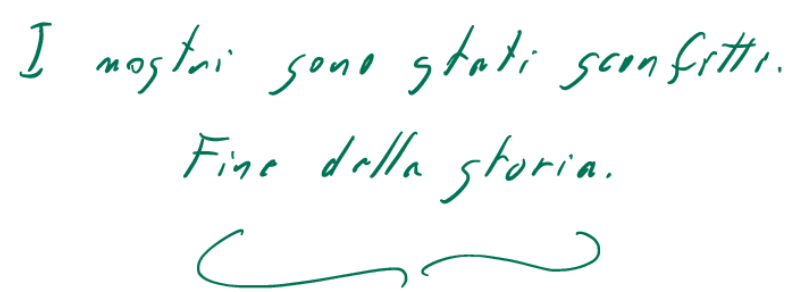
\includegraphics[width = 7.0cm]{immagini/mostri_sconfitti.png}
\end{figure}

\pagebreak

\subsection*{Esercizi}

\begin{exercise}[$|V_{\omega + \alpha}| = \beth_\alpha$]
	Definiamo $\beth_0\footnote{\;``beth''.} = \aleph_0$, $\beth_{\alpha + 1} = 2^{\beth_\alpha}$, $\beth_\lambda = \sup \{\beth_\alpha | \alpha < \lambda\}$, con $\lambda$ limite (questi cardinali definiti ricorsivamente si chiamano \vocab{beth numbers}).
	Dimostrare che $\forall \alpha \in \Ord \; |V_{\omega + \alpha}| = \beth_\alpha$.
\end{exercise}

\begin{lemma}[$\alpha \leq \beth_\alpha$]
	$\forall \alpha \in \Ord \; \alpha \leq \beth_\alpha$.\footnote{In realtà si può vedere come banale conseguenza del fatto che $\beth_\alpha : \Ord \to \Ord$ è una funzione classe strettamente crescente tra classi bene ordinate.}
\end{lemma}

\begin{proof}
	Per induzione transfinita.
	\begin{itemize}
		\item[$\boxed{\text{caso 0}}$] $0 \leq \beth_0 = \aleph_0$ è banalmente vero.
		\item[$\boxed{\text{caso $s(\alpha)$}}$] Supponiamo $\alpha < \beth_\alpha$ e osserviamo che questo significa $\alpha \leq s(\alpha) \leq \beth_\alpha$ (stiamo usando che $s(\alpha)$ è il più piccola ordinale maggiore o uguale a $\alpha$). Da ciò
		si conclude osservando che per Cantor $\beth_\alpha < 2^{\beth_\alpha} = \beth_{s(\alpha)}$, e mettendo assieme le disuguaglianze $s(\alpha) \leq \beth_{s(\alpha)}$.
		\item[$\boxed{\text{caso limite}}$] Per ipotesi induttiva abbiamo che $\alpha \leq \beth_\alpha$, per ogni $\alpha < \lambda$, essendo $x \mapsto \beth_x$ una funzione continua per costruzione, tale disuguaglianza passa quindi al sup, per cui si ottiene:
		\[ \lambda = \sup_{\alpha < \lambda} \alpha \leq \sup_{\alpha < \lambda} \beth_\alpha = \beth_\lambda
			\]
	\end{itemize}
\end{proof}

\begin{soln}
	Procediamo per induzione transfinita.
	\begin{itemize}
		\item[$\boxed{\text{caso 0}}$] $|V_{\omega + 0}| = |V_{\omega}|$, per una proposizione dimostrata sulla gerarchia, sappiamo che $\omega \subseteq V_{\omega} \implies \aleph_0 \leq |V_{\omega}|$, d'altra parte:
		\[ V_{\omega} = \bigcup_{\alpha \in \omega} V_{\alpha} \overset{\text{inclusione-esclusione}}{\implies} |V_\omega| \leq \sum_{\alpha \in \omega} |V_{\alpha}| = \max(|\omega|,|V_\alpha|)
			\]
		ma, $|V_\alpha| < \aleph_0$\footnote{Andrebbe dimostrato che, nel caso di ordinali finiti, si ha $|V_n| = 2^{V_n-1} \land |V_0| = 0$ (è una facile verifica per induzione numerabile), e ciò ci permette di dire $|V_n| \in \omega$, $\forall n \in \omega$.}, quindi abbiamo ottenuto $|V_\omega| \leq \aleph_0$. 
		\item[$\boxed{\text{caso $s(\alpha)$}}$] Supponiamo $|V_{\omega + \alpha}| = \beth_{\alpha}$ e osserviamo che $|V_{\omega + s(\alpha)}| = |\ps(V_{\omega + \alpha})| = 2^{|V_{\omega + \alpha}|}$, ora usando l'ipotesi induttiva si ottiene:
		\[ |V_{\omega + s(\alpha)}| = 2^{|V_{\omega + \alpha}|} \overset{\text{Hp. indutt.}}{=} 2^{\beth_\alpha} = \beth_{\alpha + 1}
			\]
		\item[$\boxed{\text{caso limite}}$] Per ipotesi induttiva abbiamo che $|V_{\omega + \alpha}| = \beth_\alpha$, per $\alpha < \lambda$, ci basta osservare che per definizione $V_{\omega + \alpha} \subseteq V_{\omega + \lambda}$, $\forall \alpha < \lambda$, dunque $|V_{\omega + \alpha}| \leq |V_{\omega + \lambda}|$,
		ovvero $|V_{\omega + \lambda}|$ è un maggiorante di $\{|V_{\omega + \alpha}| : \alpha < \lambda\}$, per cui:
		\[ \beth_\lambda = \sup_{\alpha < \lambda} \beth_{\alpha} \overset{\text{Hp. indutt.}}{=} \sup_{\alpha < \lambda} |V_{\omega + \alpha}| \leq |V_{\omega + \lambda}|
			\]
		mentre, per la disuguaglianza dall'alto, dato che $V_{\omega + \lambda} = \bigcup_{\alpha < \lambda} V_{\alpha}$, abbiamo:
		\begin{align*}
			|V_{\omega + \lambda}| \leq \sum_{\alpha < \lambda} |V_{\omega + \alpha}|
								   = \max\left(|\lambda|,\sup_{\alpha < \lambda} |V_{\omega + \alpha}|\right)
								   \overset{\text{Hp. indutt.}}{=} \max(|\lambda|,\beth_\lambda)
								   \overset{\text{lemma}}{=} \beth_\lambda
		\end{align*}
		in tal modo concludiamo anche il caso successore.
	\end{itemize}
\end{soln}

\begin{remark}
	Si noti che con un ragionamento analogo a quello fatto per il caso limite è possibile dimostrare che:
	\[ |V_\lambda| = \left\lvert \bigcup_{\alpha < \lambda} V_\alpha\right\rvert = \sup_{\alpha < \lambda} |V_\alpha|
		\]
	e analogamente (sfruttando il lemma di sopra):
	\[ |V_{\omega + \lambda}| = \left\lvert \bigcup_{\alpha < \lambda} V_{\omega + \alpha}\right\rvert = \sup_{\alpha < \lambda} |V_{\omega + \alpha}|
		\]
\end{remark}

\begin{exercise}[Caratterizzazione del rango]
	Dimostrare che vale la seguente identità: $\rank(x) = \sup\{\rank(y) + 1 | y \in x\}$.
\end{exercise}

\begin{soln}
	Abbiamo visto che $y \in x \implies \rank(y) < \rank (x)$, ed essendo ordinali vale $\rank(y) + 1 \leq \rank(x)$, per ogni $y \in x$, dunque $\rank(x)$ è un maggiorante dell'insieme $\{\rank(y) + 1 | y \in x\}$. Ci rimane da verificare che sia effettivamente il più piccolo maggiorante.
	Supponiamo che esista un ordinale $\alpha$ che sia maggiorante dell'insieme e allo stesso tempo $\alpha < \rank(x)$, da questo segue che $\forall y \in x \; y \in V_\alpha$, per cui $x \subseteq V_\alpha \implies x \in V_{\alpha + 1}$, pertanto, da definizione, $\rank(x) \leq \alpha$, che è assurdo.
\end{soln}

\begin{exercise}[$V_\omega$]
	Dimostrare che $V_\omega$ soddisfa tutti gli assiomi \underline{eccetto} l'\hyperref[ax7]{assioma dell'infinito}.
\end{exercise}

\begin{soln}
	Verifichiamo che valgono uno per uno gli assiomi 1-9\footnote{Avendo dimostrato che $V_*$ è ben fondata, in automatico lo è anche $V_\omega$, altrimenti si violerebbe il fatto che $V_*$ è ben fondata, pertanto non è necessario verificare che questo assioma valga in $V_\omega$.} relativizzati in $V_\omega$, eccetto l'assioma 7, ovvero l'assioma dell'infinito, ricordando che:
	\[ V_\omega = \bigcup_{\alpha < \omega} V_\alpha
		\]
	\begin{enumerate}[(1)]
		\item \textbf{\underline{Vuoto}}: \textcolor{purple}{$\exists x \in V_\omega \; \forall y \in V_\omega \; y \not \in x$} \\
		Basta prendere come $x = \emptyset \in V_1 = \ps(V_0) = \ps(\emptyset) = \{\emptyset\}$, tale insieme rispetta la proprietà richiesta e, poiché $\emptyset \in V_1 \in V_\omega$, per transitività [basta quella di $V_\omega$ stesso, ma la abbiamo comunque su tutto $V_*$] $\emptyset \in V_\omega$.
		\item \textbf{\underline{Estensionalità}}: \textcolor{purple}{$\forall a,b \in V_\omega (a = b \leftrightarrow \forall x \in V_\omega (x \in a \leftrightarrow x \in b))$} \\
		Fissati $a,b \in V_\omega$ osserviamo che, per transitività, i loro elementi sono anch'essi elementi di $V_\omega$, quindi $x \in a$ o $x \in b$ implicano $x \in V_\omega$, per cui si ha:
		\[ \forall x (x \in a \leftrightarrow x \in b) \leftrightarrow \forall x (x \in V_\omega \land (x \in a \leftrightarrow x \in b) \lor x \not \in V_\omega \land (x \in a \leftrightarrow x \in b))
			\] 
		ora il secondo elemento dell'OR è sempre falso per quanto detto prima, dunque possiamo escluderlo dall'equivalenza, e ciò ci lascia $\forall x \in V_\omega (x \in a \leftrightarrow x \in b)$.
		Dunque, per estensionalità, abbiamo l'equivalenza con $a = b$.
		\item \textbf{\underline{Separazione}}: \textcolor{purple}{$\forall A \in V_\omega \; \exists B \in V_\omega \; \forall x \in V_\omega \; x \in B \leftrightarrow (x \in A \land \varphi(x))$} \\
		Per separazione esiste l'insieme $B :=\{x \in A | x \in V_\omega \land \varphi(x)\}$. Per ipotesi $A \in V_\omega$, ovvero $A \in V_{\alpha}$, per qualche $\alpha$ ordinale, pertanto, si ha $B \subseteq A \in V_\alpha$, e per transitività $B \subseteq V_\alpha$, dunque $B \in V_{\alpha + 1}$, con $\alpha + 1 < \omega$ perché $\omega$ è limite, quindi otteniamo che $B \in V_\omega$.
		\item \textbf{\underline{Paio}}: \textcolor{purple}{$\forall a,b \in V_\omega \; \exists B \in V_\omega \; \forall x \in V_\omega \; x \in B \leftrightarrow (x = a \lor x = b)$} \\
		Dati $a,b \in V_\omega$, abbiamo che $a \in V_\alpha$ e $b \in V_\beta$, e, WLOG, possiamo assumere $\alpha \leq \beta$, allora $a,b \in V_\beta$, da cui necessariamente il paio, che esiste per l'assioma non relativizzato, è nelle parti di $V_\beta$, $\{a,b\} \in \ps(V_\beta) = V_{\beta+1}$, dove naturalmente $\beta + 1 < \omega$, e in questo modo, per transitività, si ottiene che $\{a,b\} \in V_\omega$.
		\item \textbf{\underline{Unione}}: \textcolor{purple}{$\forall A \in V_\omega \; \exists B \in V_\omega \; \forall x \in V_\omega \; x \in B \leftrightarrow \exists y \in A \; x \in y$} \\
		Sia $A \in V_\alpha$, per qualche ordinale $\alpha < \omega$, per transitività, $A \subseteq V_\alpha$, ciò significa che $\bigcup A$, che esiste per unione non relativizzata, ed è l'insieme degli elementi degli elementi di $A \subseteq V_\alpha$, è a sua volta contenuto in $V_\alpha$ (perché gli elementi degli elementi di $A$ per transitività sono a loro volta elementi di $V_\alpha$), dunque
		$\bigcup A \subseteq V_\alpha\footnote{Osserviamo che in generale $A \subseteq B \implies \bigcup A \subseteq B \iff B$ è transitivo.} \implies \bigcup A \in \ps(V_\alpha) = V_{\alpha+1}$, e quindi come prima, per transitività si conclude che $\bigcup A \in V_\omega$.
		\item \textbf{\underline{Parti}}: \textcolor{purple}{$\forall A \in V_\omega \; \exists B \in V_\omega \; \forall x \in V_\omega \; x \in B \leftrightarrow x \subseteq B$} \\
		Sia $A \in V_\alpha$, quindi per transitività $A \subseteq V_{\alpha}$, allora si ha $\ps(A) \subseteq \ps(V_\alpha) = V_{\alpha + 1}$, dove le parti esistono per l'assioma non relativizzato, quindi $\ps(A) \in \ps(V_{s(\alpha)}) = V_{\alpha + 2}$, per cui $\ps(A) \in V_\omega$.
		\item \textbf{\underline{Rimpiazzamento}}: \textcolor{purple}{$F : V_\omega \rightarrow V_\omega$ funzione classe e $X \in V_\omega \rightarrow F[X] \in V_\omega$} \\
		Sia $X \in V_\alpha$, per transitività, $\forall x \in X \to x \in V_\alpha$, cioè $X \subseteq V_\alpha$, dunque è ben definita $F[X]$ in quanto possiamo fare $F(a)$ per ogni $a \in X$, perché, come detto, $a \in V_\alpha \in V_\omega$. A questo punto, definiamo $\alpha_a :=\min\{\gamma \in \omega | F(a) \in V_\gamma\}$ e $\beta :=\sup\{\alpha_a\}_{a \in X}$, e osserviamo che l'insieme su cui stiamo prendendo il sup è finito, in quanto $|F[X]| \leq |X| \leq |V_\alpha| = 2^{|V_{\alpha - 1}|}$\footnote{Osserviamo
		sempre che ciò esclude il caso banale, e che andrebbe dimostrato che $|V_n| = 2^{|V_{n-1}|} \land |V_0| = 0$ (è una facilissima induzione numerabile) per poter assicurare la finitezza di ciò che stiamo facendo.} (e qui stiamo usando che $\alpha \in \omega$),
		dunque ha proprio un massimo $\beta \in \omega$, per cui $F(a) \in V_\beta$, $\forall a \in X$, ovvero $F[x] \subseteq V_\beta \implies F[X] \in V_{\beta + 1}$, e per transitività $F[X] \in V_\omega$.
		\item \textbf{\underline{Scelta}}: \textcolor{purple}{$\forall X \in V_\omega (\forall y \in X \; y \ne \emptyset)\footnote{Cioè se $\emptyset \not \in X$.} \rightarrow \exists f \in V_\omega$ funzione di scelta su $X$} \\
		Sia $f$ una funzione di scelta su $X \in V_\alpha$, che esiste per AC, sappiamo che $f \in {}^X\bigcup X$, cioè $f \in \ps\left(X \times \bigcup X\right)$. Ricordando che $X \times \bigcup X \subseteq \ps(\ps(X \cup \bigcup X))$ e che $X \subseteq V_\alpha$ (che vale per transitività) implica $\bigcup X \subseteq V_\alpha$, abbiamo:
		\[ X \cup \bigcup X \subseteq V_\alpha \implies f \in \ps\left(\ps\left(\ps\left(X \cup \bigcup X\right)\right)\right) \subseteq \ps(\ps(\ps(V_\alpha))) = V_{\alpha + 3}
			\]
		naturalmente $\alpha + 3 < \omega$, quindi $V_{\alpha + 3} \in V_\omega$, e per transitività si ha che $f \in V_\omega$.
	\end{enumerate}
	Infine, non ci resta che verificare che $V_\omega$ non soddisfa l'assioma dell'infinito, in primis osserviamo che $\omega \not \in V_\omega$, in quanto $\rank(\omega) = \omega$, inoltre se esistesse un insieme induttivo $X \in V_\omega$, poiché avevamo definito $\omega$ come l'intersezione della classe di tutti gli insiemi induttivi, avremmo che $\omega \subseteq X$, e siccome $X \in V_\omega \implies X \in V_\alpha$, per $\alpha < \omega$,
	si ha che $\omega \in V_{\alpha + 1} \in V_\omega \implies \omega \in V_\omega \;\lightning$.  
\end{soln}

\begin{remark}[Esistenza di insiemi infiniti]
	L'esercizio appena risolto ha come conseguenza che l'esistenza di un insieme induttivo è indipendente dagli assiomi della ZFC ad eccezione dell'assioma dell'infinito, e ciò ci dà appunto una giustificazione all'introduzione di tale assioma. In particolare senza questo insieme non possiamo costruire $\omega$ e quindi nessun altro insieme infinito (potremmo costruire solo insiemi ereditariamente finiti usando gli altri assiomi), pertanto 
	si capisce ancora meglio perché l'assioma dell'infinito ci garantisce la possibilità di definire insiemi infiniti.
\end{remark}

\begin{exercise}[$V_{\omega + \omega}$]
	Dimostrare che $V_{\omega + \omega}$ soddisfa tutti gli assiomi \underline{eccetto} l'\hyperref[ax8]{assioma del rimpiazzamento}.
\end{exercise}

\begin{soln}
	Verifichiamo che valgono uno per uno gli assiomi 1-9\footnote{Esattamente come per $V_\omega$ non è necessario dimostrare che valga buona fondazione.} relativizzati in $V_{\omega + \omega}$, eccetto l'assioma 8, ovvero l'assioma del rimpiazzamento, ricordando che:
	\[ V_{\omega + \omega} = \bigcup_{\alpha < \omega} V_{\omega + \alpha}
		\]
	\begin{enumerate}[(1)]
		\item \textbf{\underline{Vuoto}}: \textcolor{purple}{$\exists x \in V_{\omega + \omega} \; \forall y \in V_{\omega + \omega} \; y \not \in x$} \\
		Basta prendere come $x = \emptyset \in V_1 = \ps(V_0) = \ps(\emptyset) = \{\emptyset\}$, tale insieme rispetta la proprietà richiesta e, poiché $\emptyset \in V_1 \in V_{\omega + \omega}$, per transitività [basta quella di $V_{\omega + \omega}$ stesso, ma la abbiamo comunque su tutto $V_*$] $\emptyset \in V_{\omega + \omega}$.
		\item \textbf{\underline{Estensionalità}}: \textcolor{purple}{$\forall a,b \in V_{\omega + \omega} (a = b \leftrightarrow \forall x \in V_{\omega + \omega} (x \in a \leftrightarrow x \in b))$} \\
		Fissati $a,b \in V_{\omega + \omega}$ osserviamo che, per transitività, i loro elementi sono anch'essi elementi di $V_{\omega + \omega}$, quindi $x \in a$ o $x \in b$ implicano $x \in V_{\omega + \omega}$, per cui si ha:
		\[ \forall x (x \in a \leftrightarrow x \in b) \leftrightarrow \forall x (x \in V_{\omega + \omega} \land (x \in a \leftrightarrow x \in b) \lor x \not \in V_{\omega + \omega} \land (x \in a \leftrightarrow x \in b))
			\] 
		ora il secondo elemento dell'OR è sempre falso per quanto detto prima, dunque possiamo escluderlo dall'equivalenza, e ciò ci lascia $\forall x \in V_{\omega + \omega} (x \in a \leftrightarrow x \in b)$.
		Dunque, per estensionalità, abbiamo l'equivalenza con $a = b$.
		\item \textbf{\underline{Separazione}}: \textcolor{purple}{$\forall A \in V_{\omega + \omega} \; \exists B \in V_{\omega + \omega} \; \forall x \in V_{\omega + \omega} \; x \in B \leftrightarrow (x \in A \land \varphi(x))$} \\
		Per separazione esiste l'insieme $B :=\{x \in A | x \in V_{\omega + \omega} \land \varphi(x)\}$. Per ipotesi $A \in V_{\omega + \omega}$, ovvero $A \in V_{\alpha}$, per qualche $\alpha$ ordinale, pertanto, si ha $B \subseteq A \in V_\alpha$, e per transitività $B \subseteq V_\alpha$, dunque $B \in V_{\alpha + 1}$, con $\alpha + 1 < {\omega + \omega}$ perché ${\omega + \omega}$ è limite, quindi otteniamo che $B \in V_{\omega + \omega}$.
		\item \textbf{\underline{Paio}}: \textcolor{purple}{$\forall a,b \in V_{\omega + \omega} \; \exists B \in V_{\omega + \omega} \; \forall x \in V_{\omega + \omega} \; x \in B \leftrightarrow (x = a \lor x = b)$} \\
		Dati $a,b \in V_{\omega + \omega}$, abbiamo che $a \in V_\alpha$ e $b \in V_\beta$, e, WLOG, possiamo assumere $\alpha \leq \beta$, allora $a,b \in V_\beta$, da cui necessariamente il paio, che esiste per l'assioma non relativizzato, è nelle parti di $V_\beta$, $\{a,b\} \in \ps(V_\beta) = V_{\beta+1}$, dove naturalmente $\beta + 1 < {\omega + \omega}$, e in questo modo, per transitività, si ottiene che $\{a,b\} \in V_{\omega + \omega}$.
		\item \textbf{\underline{Unione}}: \textcolor{purple}{$\forall A \in V_{\omega + \omega} \; \exists B \in V_{\omega + \omega} \; \forall x \in V_{\omega + \omega} \; x \in B \leftrightarrow \exists y \in A \; x \in y$} \\
		Sia $A \in V_\alpha$, per qualche ordinale $\alpha < \omega + \omega$, per transitività, $A \subseteq V_\alpha$, ciò significa che $\bigcup A$, che esiste per unione non relativizzata, ed è l'insieme degli elementi degli elementi di $A \subseteq V_\alpha$, è a sua volta contenuto in $V_\alpha$ (perché gli elementi degli elementi di $A$ per transitività sono a loro volta elementi di $V_\alpha$), dunque
		$\bigcup A \subseteq V_\alpha\footnote{Osserviamo che in generale $A \subseteq B \implies \bigcup A \subseteq B \iff B$ è transitivo.} \implies \bigcup A \in \ps(V_\alpha) = V_{\alpha+1}$, e quindi come prima, per transitività si conclude che $\bigcup A \in V_{\omega + \omega}$.
		\item \textbf{\underline{Parti}}: \textcolor{purple}{$\forall A \in V_{\omega + \omega} \; \exists B \in V_{\omega + \omega} \; \forall x \in V_{\omega + \omega} \; x \in B \leftrightarrow x \subseteq B$} \\
		Sia $A \in V_\alpha$, quindi per transitività $A \subseteq V_{\alpha}$, allora si ha $\ps(A) \subseteq \ps(V_\alpha) = V_{\alpha + 1}$, dove le parti esistono per l'assioma non relativizzato, quindi $\ps(A) \in \ps(V_{s(\alpha)}) = V_{\alpha + 2}$, per cui $\ps(A) \in V_{\omega + \omega}$.
		\item \textbf{\underline{Infinito}}: \textcolor{purple}{$\exists X \in V_{\omega + \omega} \; \emptyset \in X \land \forall x \in X \to x \cup \{x\} \in X$} \\
		Basta prendere $X = \omega \in V_{\omega + 1}$, con $V_{\omega + 1} \in V_{\omega + \omega}$, e per transitività $X \in V_{\omega + \omega}$.
		\item \textbf{\underline{Scelta}}: \textcolor{purple}{$\forall X \in V_{\omega + \omega} (\forall y \in X \; y \ne \emptyset)\footnote{Cioè se $\emptyset \not \in X$.} \rightarrow \exists f \in V_{\omega + \omega}$ funzione di scelta su $X$} \\
		Sia $f$ una funzione di scelta su $X \in V_\alpha$, che esiste per AC, sappiamo che $f \in {}^X\bigcup X$, cioè $f \in \ps\left(X \times \bigcup X\right)$. Ricordando che $X \times \bigcup X \subseteq \ps(\ps(X \cup \bigcup X))$ e che $X \subseteq V_\alpha$ (che vale per transitività) implica $\bigcup X \subseteq V_\alpha$, abbiamo:
		\[ X \cup \bigcup X \subseteq V_\alpha \implies f \in \ps\left(\ps\left(\ps\left(X \cup \bigcup X\right)\right)\right) \subseteq \ps(\ps(\ps(V_\alpha))) = V_{\alpha + 3}
			\]
		naturalmente $\alpha + 3 < {\omega + \omega}$, quindi $V_{\alpha + 3} \in V_{\omega + \omega}$, e per transitività si ha che $f \in V_{\omega + \omega}$.
	\end{enumerate}
	Infine, dobbiamo dimostrare che non vale l'assioma del rimpiazzamento, osserviamo in primis che l'argomento utilizzato per dimostrare la validità di questo assioma per $V_{\omega}$ qui fallisce in quanto $\beta$ non è necessariamente finito, ed in particolare potrebbe accadere che $\beta = \omega + \omega$, il che implicherebbe $F[X] \in V_{\omega + \omega + 1}$, e ciò fa fallire la dimostrazione in questo caso.
	Supponiamo per assurdo che $V_{\omega + \omega}$ soddisfi l'assioma del rimpiazzamento, allora esiste l'insieme $\omega + \omega \in V_{\omega + \omega}$, per la dimostrazione vista che ogni classe di isomorfismo ha associato un ordinale (ed in particolare ci basta prendere l'ordinale associato all'insieme di vuoto e $\omega$ in un numero finito di singoletti che abbiamo visto in un esercizio nella sezione sugli ordinali),
	ma ciò è assurdo in quanto, per la proprietà del rango di un ordinale, si ha $\rank(\omega + \omega) = \omega + \omega \implies \omega + \omega \not \in V_{\omega + \omega}$.
\end{soln}

\begin{exercise}[Rimpiazzamento $\implies \exists\, \omega + \omega$]
	Dimostrare che l'esistenza dell'ordinale $\omega + \omega$ non segue dagli assiomi della teoria degli insiemi, \underline{escluso} l'\hyperref[ax8]{assioma del rimpiazzamento}, a patto 
	che questi non si contraddicano.
\end{exercise}

\begin{soln}
	Se per assurdo l'esistenza di $\omega + \omega$ seguisse dagli assiomi della ZFC tranne rimpiazzamento, assumendo che sono coerenti (e quindi non si contraddicono, altrimenti potremmo dimostrare qualsiasi cosa),
	allora un tale ordinale esisterebbe anche in $V_{\omega + \omega}$, visto che abbiamo dimostrato che in tale insieme valgono tutti gli assiomi tranne appunto rimpiazzamento.
	Tuttavia, sappiamo che $\rank(\omega + \omega) = \omega + \omega$, quindi $\omega + \omega \not \in V_{\omega + \omega}$, pertanto ciò è assurdo. Abbiamo quindi dimostrato che l'esistenza dell'ordinale $\omega + \omega$ è indipendente dagli assiomi della ZFC, escluso il rimpiazzamento.
\end{soln}

\begin{exercise}[$V_\kappa$ - $\kappa$ fortemente inaccessibile]
	Dimostrare che, se $\kappa$ è [fortemente] inaccessibile, allora tutti gli assiomi della teoria degli insiemi valgono in $V_\kappa$.
\end{exercise}

\begin{soln}
	Ricordiamo innanzitutto che $\kappa$ fortemente inaccessibile significa che $\kappa$ è un ordinale iniziale (quindi limite) regolare, $\cof(\kappa) = \kappa$, ed è limite forte, cioè $\aleph_0 < \kappa$ e $\forall \alpha \; \aleph_\alpha < \kappa \to 2^{\aleph_\alpha} < \kappa$. Ciò significa che $\omega < \kappa \to V_\omega \in V_\kappa$.\footnote{Come al solito $V_*$ è ben fondata, dunque non è necessario verificare buona fondazione in $V_\kappa$, in quanto è già dato.}
	\begin{enumerate}[(1)]
		\item \textbf{\underline{Vuoto}}: \textcolor{purple}{$\exists x \in V_\kappa \; \forall y \in V_\kappa \; y \not \in x$} \\
		Basta prendere come $x = \emptyset \in V_1 = \ps(V_0) = \ps(\emptyset) = \{\emptyset\}$, tale insieme rispetta la proprietà richiesta e, poiché $\emptyset \in V_1 \in V_\kappa$, per transitività [basta quella di $V_\kappa$ stesso, ma la abbiamo comunque su tutto $V_*$] $\emptyset \in V_\kappa$.
		\item \textbf{\underline{Estensionalità}}: \textcolor{purple}{$\forall a,b \in V_\kappa (a = b \leftrightarrow \forall x \in V_\kappa (x \in a \leftrightarrow x \in b))$} \\
		Fissati $a,b \in V_\kappa$ osserviamo che, per transitività, i loro elementi sono anch'essi elementi di $V_\kappa$, quindi $x \in a$ o $x \in b$ implicano $x \in V_\kappa$, per cui si ha:
		\[ \forall x (x \in a \leftrightarrow x \in b) \leftrightarrow \forall x (x \in V_\kappa \land (x \in a \leftrightarrow x \in b) \lor x \not \in V_\kappa \land (x \in a \leftrightarrow x \in b))
			\] 
		ora il secondo elemento dell'OR è sempre falso per quanto detto prima, dunque possiamo escluderlo dall'equivalenza, e ciò ci lascia $\forall x \in V_\kappa (x \in a \leftrightarrow x \in b)$.
		Dunque, per estensionalità, abbiamo l'equivalenza con $a = b$.
		\item \textbf{\underline{Separazione}}: \textcolor{purple}{$\forall A \in V_\kappa \; \exists B \in V_\kappa \; \forall x \in V_\kappa \; x \in B \leftrightarrow (x \in A \land \varphi(x))$} \\
		Per separazione esiste l'insieme $B :=\{x \in A | x \in V_\kappa \land \varphi(x)\}$. Per ipotesi $A \in V_\kappa$, ovvero $A \in V_{\alpha}$, per qualche $\alpha$ ordinale, pertanto, si ha $B \subseteq A \in V_\alpha$, e per transitività $B \subseteq V_\alpha$, dunque $B \in V_{\alpha + 1}$, con $\alpha + 1 < \kappa$ perché $\kappa$ è limite, quindi otteniamo che $B \in V_\kappa$.
		\item \textbf{\underline{Paio}}: \textcolor{purple}{$\forall a,b \in V_\kappa \; \exists B \in V_\kappa \; \forall x \in V_\kappa \; x \in B \leftrightarrow (x = a \lor x = b)$} \\
		Dati $a,b \in V_\kappa$, abbiamo che $a \in V_\alpha$ e $b \in V_\beta$, e, WLOG, possiamo assumere $\alpha \leq \beta$, allora $a,b \in V_\beta$, da cui necessariamente il paio, che esiste per l'assioma non relativizzato, è nelle parti di $V_\beta$, $\{a,b\} \in \ps(V_\beta) = V_{\beta+1}$, dove naturalmente $\beta + 1 < \kappa$, e in questo modo, per transitività, si ottiene che $\{a,b\} \in V_\kappa$.
		\item \textbf{\underline{Unione}}: \textcolor{purple}{$\forall A \in V_\kappa \; \exists B \in V_\kappa \; \forall x \in V_\kappa \; x \in B \leftrightarrow \exists y \in A \; x \in y$} \\
		Sia $A \in V_\alpha$, per qualche ordinale $\alpha < \kappa$, per transitività, $A \subseteq V_\alpha$, ciò significa che $\bigcup A$, che esiste per unione non relativizzata, ed è l'insieme degli elementi degli elementi di $A \subseteq V_\alpha$, è a sua volta contenuto in $V_\alpha$ (perché gli elementi degli elementi di $A$ per transitività sono a loro volta elementi di $V_\alpha$), dunque
		$\bigcup A \subseteq V_\alpha\footnote{Osserviamo che in generale $A \subseteq B \implies \bigcup A \subseteq B \iff B$ è transitivo.} \implies \bigcup A \in \ps(V_\alpha) = V_{\alpha+1}$, e quindi come prima, per transitività si conclude che $\bigcup A \in V_\kappa$.
		\item \textbf{\underline{Parti}}: \textcolor{purple}{$\forall A \in V_\kappa \; \exists B \in V_\kappa \; \forall x \in V_\kappa \; x \in B \leftrightarrow x \subseteq B$} \\
		Sia $A \in V_\alpha$, quindi per transitività $A \subseteq V_{\alpha}$, allora si ha $\ps(A) \subseteq \ps(V_\alpha) = V_{\alpha + 1}$, dove le parti esistono per l'assioma non relativizzato, quindi $\ps(A) \in \ps(V_{s(\alpha)}) = V_{\alpha + 2}$, per cui $\ps(A) \in V_\kappa$.
		\item \textbf{\underline{Infinito}}: \textcolor{purple}{$\exists X \in V_\kappa \; \emptyset \in X \land \forall x \in X \to x \cup \{x\} \in X$} \\
		Basta prendere $X = \omega \in V_{\omega + 1}$, con $V_{\omega + 1} \in V_\kappa$, e per transitività $X \in V_\kappa$.
		\item \textbf{\underline{Scelta}}: \textcolor{purple}{$\forall X \in V_\kappa (\forall y \in X \; y \ne \emptyset)\footnote{Cioè se $\emptyset \not \in X$.} \rightarrow \exists f \in V_\kappa$ funzione di scelta su $X$} \\
		Sia $f$ una funzione di scelta su $X \in V_\alpha$, che esiste per AC, sappiamo che $f \in {}^X\bigcup X$, cioè $f \in \ps\left(X \times \bigcup X\right)$. Ricordando che $X \times \bigcup X \subseteq \ps(\ps(X \cup \bigcup X))$ e che $X \subseteq V_\alpha$ (che vale per transitività) implica $\bigcup X \subseteq V_\alpha$, abbiamo:
		\[ X \cup \bigcup X \subseteq V_\alpha \implies f \in \ps\left(\ps\left(\ps\left(X \cup \bigcup X\right)\right)\right) \subseteq \ps(\ps(\ps(V_\alpha))) = V_{\alpha + 3}
			\]
		naturalmente $\alpha + 3 < \kappa$, quindi $V_{\alpha + 3} \in V_\kappa$, e per transitività si ha che $f \in V_\kappa$.
		\item \textbf{\underline{Rimpiazzamento}}: \textcolor{purple}{$F : V_\kappa \rightarrow V_\kappa$ funzione classe e $X \in V_\kappa \rightarrow F[X] \in V_\kappa$} \\
		Sia $X \in V_\alpha$, con $\alpha < \kappa$, per transitività, $\forall x \in X \to x \in V_\alpha$, cioè $X \subseteq V_\alpha$, dunque è ben definita $F[X]$ in quanto possiamo fare $F(a)$ per ogni $a \in X$, perché, come detto, $a \in V_\alpha \in V_\kappa$, inoltre $F(a) \in V_\kappa$ per definizione di $F$. A questo punto, definiamo $\alpha_a :=\min\{\gamma \in \kappa | F(a) \in V_\gamma\footnote{Per la precisione, per definizione di $F$ e $V_\kappa$, si ha $F(a) \in V_\kappa \to F(a) \in V_\gamma$, $\gamma \in \kappa$. Dunque
		gli $\alpha_a$ sono tutti strettamente minori di $\kappa$, il problema è che potrebbe non esserlo il loro sup.}\}$ e $\beta :=\sup\{\alpha_a\}_{a \in X}$, essendo 
		$F : V_\kappa \to V_\kappa$ abbiamo che $\beta \leq \kappa$, se escludiamo che $\beta = \kappa$, allora $\beta < \kappa$, per cui, essendo $\kappa$ limite, $\beta + 1 < \kappa$ ed a questo punto abbiamo $F[X] \subseteq V_\beta \implies F[X] \in V_{\beta + 1} \in V_\kappa$ e si conclude per transitività.\\
		Ci rimane quindi da escludere che $\beta = \kappa$. Per ipotesi sappiamo che $\beta = \kappa = \cof(\kappa)$, osserviamo che $\{\alpha_a | a \in X\}$ è un sottoinsieme cofinale di $\beta$ praticamente perché $\beta$ è l'estremo superiore di questo insieme (dunque la definizione di sottoinsieme cofinale è verificata immediatamente),
		inoltre si ha $|\{\alpha_a | a \in X\}| \leq |X|$ (ci basta considerare la mappa $x \mapsto \alpha_x$ che è surgettiva\footnote{Per la precisione $X \twoheadrightarrow s[\rank[X]] : x \to \alpha_x$, dove l'insieme d'arrivo è un insieme per rimpiazzamento non relativizzato.}), a questo punto, se verifichiamo che $|X| < \kappa$ abbiamo un assurdo:
		\[ \kappa = \cof(\kappa) = \cof(\beta) \leq |X| < \kappa \; \lightning
			\]
		Per dimostrare l'ultima cosa ci basta dimostrare per induzione transfinita che $|V_\alpha| < \kappa$, $\forall \alpha < \kappa$, da cui si ha $X \subseteq V_\alpha \implies |X| \leq |V_\alpha| < \kappa$, $\alpha < \kappa$.
		\begin{itemize}
			\item[$\boxed{\text{caso 0}}$] È ovvio che $0 = |V_0| < \kappa$, in quanto $\kappa > \aleph_0$ poiché limite forte. 
			\item[$\boxed{\text{caso successore}}$] Supponiamo $|V_\alpha| < \kappa$, a questo punto $|V_{\alpha + 1}| = 2^{|V_\alpha|} < \kappa$, dove l'ultima disuguaglianza vale perché $\kappa$ è limite forte.
			\item[$\boxed{\text{caso limite}}$] Abbiamo per ipotesi $|V_\alpha| < \kappa$, per $\alpha < \lambda < \kappa$, dunque:
			\[ |V_\lambda| = \left\lvert \bigcup_{\alpha < \lambda} V_\alpha\right\rvert \leq \sum_{\alpha < \lambda} |V_\alpha| = |\lambda| \cdot \sup_{\alpha < \lambda} |V_\alpha| \leq \kappa
				\]
			ora, essendo che $|\lambda| < \kappa$ e per ipotesi induttiva $|V_\alpha| < \kappa$, con $\alpha < \kappa$, se la somma facesse $\kappa$, avremmo trovato una stima dall'alto per la cofinalità, data da $|\lambda| < \kappa$, ma $\cof(\kappa) = \kappa$, dunque ciò è assurdo, e la somma è $<\kappa$.
		\end{itemize}
	\end{enumerate}
\end{soln}

\begin{remark}[Alternativa per il rimpiazzamento in $V_\kappa$]
	Il punto chiave della dimostrazione della validità dell'assioma del rimpiazzamento in $V_\kappa$ è l'assurdo ottenuto violando il fatto che $\kappa$ sia regolare, questa cosa può essere fatta anche ragionando sulla prima definizione data di cofinalità, così da escludere che $\beta = \kappa$.\\
	Per verificare che $\beta < \kappa$ è sufficiente verificare che $|\beta| < \kappa$, essendo $\kappa$ un ordinale iniziale, e, essendo $\beta = \bigcup_{a \in X} \alpha_a$ si ha:
	\[ |\beta| \leq \sum_{a \in X} |\alpha_a| = |X| \cdot \sup_{a \in X} |\alpha_a|
		\]
	a questo punto, come nella dimostrazione sopra, sappiamo che $|X| < \kappa$, per cui, se la somma sopra fosse uguale a $\kappa$, allora il sup sarebbe uguale a $\kappa$, ma $|\alpha_a| < \kappa$, $\forall a \in X$, in quanto $a \in X$, per cui avremmo ottenuto una stima dall'alto per la cofinalità (v.1) di $\kappa$ (cioè avremmo ottenuto che $\kappa$ si può scrivere come somma di cose più piccole
	un numero di volte $< \kappa$) che è assurda in quanto $\kappa = \cof(\kappa) \leq |X| < \kappa$. Segue quindi che la somma è minore strettamente di $\kappa$, dunque $|\beta| < \kappa$.\footnote{Idea proposta da Rubens Alessio Martino.}
\end{remark}

\begin{exercise}[ZFC $\notimplies$ esiste un cardinale fortemente inaccessibile]
	Dimostrare che, se la teoria degli insiemi è coerente, allora non dimostra l'esistenza di un cardinale [fortemente] inaccessibile.
\end{exercise}

\begin{soln}
	Se per assurdo l'esistenza di un cardinale fortemente inaccessibile $\kappa$ seguisse dagli assiomi della ZFC, assumendo che sono coerenti (e quindi non si contraddicono, altrimenti potremmo dimostrare qualsiasi cosa), allora,
	per quanto dimostrato nell'esercizio precedente, l'esistenza di $\kappa$ seguirebbe anche in $V_\kappa$, avendo dimostrato che anche qui valgono tutti gli assiomi. Tuttavia ciò è assurdo in quanto $\rank(\kappa) = \kappa$ ($\kappa$ è un cardinale, dunque un ordinale iniziale, quindi vale anche per lui la proprietà del rango degli ordinali), quindi 
	$\kappa \not \in V_\kappa$, pertanto l'esistenza di un cardinale fortemente inaccessibile è indipendente dagli assiomi della ZFC.
\end{soln}

\begin{remark}[$V_\kappa$ - $\kappa$ debolmente inaccessibile]
	Si potrebbe essere tentati di dimostrare che anche nel caso di $V_\kappa$, con $\kappa$ cardinale debolmente inaccessibile siano verificati tutti gli assiomi della ZFC, ed in effetti lo sono tutti ad eccezione del rimpiazzamento. In particolare, non solo la dimostrazione fatta nel caso di $\kappa$ fortemente inaccessibile non funziona (poiché avevamo usato l'ipotesi di limite forte),
	ma si verifica addirittura che rimpiazzamento non può proprio valere in $V_\kappa$, con $\kappa$ debolmente inaccessibile.
\end{remark}

\begin{proof}
	Sia $V_{\kappa}$, con $\kappa$ cardinale debolmente inaccessibile, essendo che $\kappa$ non è limite forte, esiste almeno un cardinale $\lambda < \kappa$, tale che $2^{\lambda} \geq \kappa$. A questo punto 
	ci basta considerare l'Hartogs $H(2^{\lambda}) > 2^{\lambda}$, se valesse il rimpiazzamento si avrebbe che $H(2^{\lambda}) \in V_{\kappa}$, ma, d'altra parte, si ha:
	\[ \kappa \leq 2^{\lambda} < H(2^\lambda) \in V_{\kappa} \implies \kappa \in H(2^\lambda) \in V_{\kappa} \implies \kappa \in V_{\kappa} \; \lightning
		\]
\end{proof}

\begin{remark}
	[Esistenza di un cardinale debolmente inaccessibile in ZFC]
	L'esistenza di cardinali debolmente inaccessibili, analogamente a quella dei fortemente inaccessibili, è indipendente dalla ZFC, ma non possiamo dimostrarlo usando solo la gerarchia di Von Neumann come fatto nel caso dei fortemente inaccessibili per il motivo appena visto.
\end{remark}